%%%%%%%%%%%%%%%%%%%%%%%%%%%%%%%%%
% Set-theoretic operations on Bernoulli sets
%%%%%%%%%%%%%%%%%%%%%%%%%%%%%%%%%

\section{Set-theoretic operations}
\label{sec:set_theory}
In this section, we derive the error rates of Bernoulli sets under the
standard set-theoretic operations: complement, union, intersection, and set
difference.
Throughout, we assume that the Bernoulli sets $\tilde{A}_1$ and
$\tilde{A}_2$ approximate objective sets $A_1$ and $A_2$ respectively over
a common finite universal set $U$ with cardinality $u = |U|$.
The Bernoulli set $\tilde{A}_i$ has false positive rate $\fprate_i$ and
false negative rate $\fnrate_i$ for $i \in \{1,2\}$.
By the axioms of the Bernoulli set model, the membership errors of distinct
elements are independent.

\begin{assumption}[Cross-set independence]
\label{asm:cross_set_indep}
The Bernoulli sets $\tilde{A}_1$ and $\tilde{A}_2$ are constructed using independent randomness: for all $x \in U$, the error indicators $\mathbf{1}_{\tilde{A}_1}(x) \neq \mathbf{1}_{A_1}(x)$ and $\mathbf{1}_{\tilde{A}_2}(x) \neq \mathbf{1}_{A_2}(x)$ are independent.
\end{assumption}

\subsection{Complement}
\label{sec:complement}
The complement operation exchanges the roles of positives and negatives.
Accordingly, false positives become false negatives and vice versa.

\begin{theorem}[Complement error rates]
\label{thm:complement_rates}
Let $\tilde{A}$ be a Bernoulli set approximating $A$ with false positive
rate $\fprate$ and false negative rate $\fnrate$.
Then the complement $\SetComplement[\tilde{A}]$ is a Bernoulli set
approximating $A^c$ with false positive rate $\fnrate$ and false negative
rate $\fprate$.
\end{theorem}
\begin{proof}
The positives of $A^c$ are exactly the negatives of $A$, and the negatives
of $A^c$ are exactly the positives of $A$.

A false positive of $\SetComplement[\tilde{A}]$ with respect to $A^c$
occurs when an element $x \notin A^c$ (i.e., $x \in A$) satisfies
$x \in \SetComplement[\tilde{A}]$, which holds if and only if
$x \notin \tilde{A}$.
Since $x \in A$, the event $x \notin \tilde{A}$ is a false negative of
$\tilde{A}$, which occurs with probability $\fnrate$.
Therefore the false positive rate of $\SetComplement[\tilde{A}]$ with
respect to $A^c$ is $\fnrate$.

A false negative of $\SetComplement[\tilde{A}]$ with respect to $A^c$
occurs when an element $x \in A^c$ (i.e., $x \notin A$) satisfies
$x \notin \SetComplement[\tilde{A}]$, which holds if and only if
$x \in \tilde{A}$.
Since $x \notin A$, the event $x \in \tilde{A}$ is a false positive of
$\tilde{A}$, which occurs with probability $\fprate$.
Therefore the false negative rate of $\SetComplement[\tilde{A}]$ with
respect to $A^c$ is $\fprate$.
\end{proof}

\begin{remark}
\Cref{thm:complement_rates} establishes that complementation maps positive
Bernoulli sets ($\fnrate = 0$) to negative Bernoulli sets ($\fprate = 0$)
and vice versa.
\end{remark}

\subsection{Union}
\label{sec:union}
We derive the false positive and false negative rates of the union
$\tilde{A}_1 \cup \tilde{A}_2$ as a Bernoulli set approximating
$A_1 \cup A_2$.

\begin{theorem}[Union false positive rate]
\label{thm:union_fprate}
The union $\tilde{A}_1 \cup \tilde{A}_2$ has false positive rate
\begin{equation}
\label{eq:union_fpr}
\fprate = 1 - (1 - \fprate_1)(1 - \fprate_2)
\end{equation}
with respect to $A_1 \cup A_2$.
\end{theorem}
\begin{proof}
Let $x \notin A_1 \cup A_2$.
Then $x \notin A_1$ and $x \notin A_2$, so $x$ is a negative of both
$A_1$ and $A_2$.
A false positive of the union occurs when
$x \in \tilde{A}_1 \cup \tilde{A}_2$, i.e., when
$x \in \tilde{A}_1$ or $x \in \tilde{A}_2$ (or both).
By the independence of errors across the two Bernoulli sets (\cref{asm:cross_set_indep}),
\begin{align}
\Prob{x \in \tilde{A}_1 \cup \tilde{A}_2 \Given x \notin A_1 \cup A_2}
&= 1 - \Prob{x \notin \tilde{A}_1 \cup \tilde{A}_2
    \Given x \notin A_1 \cup A_2} \\
&= 1 - \Prob{x \notin \tilde{A}_1 \Given x \notin A_1}\,
       \Prob{x \notin \tilde{A}_2 \Given x \notin A_2} \\
&= 1 - (1 - \fprate_1)(1 - \fprate_2).
\end{align}
Since this probability is the same for every negative of $A_1 \cup A_2$,
the false positive rate of the union is
$\fprate = 1 - (1 - \fprate_1)(1 - \fprate_2)$.
\end{proof}

\begin{theorem}[Union false negative rate]
\label{thm:union_fnrate}
The union $\tilde{A}_1 \cup \tilde{A}_2$ has false negative rate
\begin{equation}
\label{eq:union_fnr}
\fnrate = w_1 \fnrate_1 (1 - \fprate_2)
        + w_2 \fnrate_2 (1 - \fprate_1)
        + w_3 \fnrate_1 \fnrate_2
\end{equation}
with respect to $A_1 \cup A_2$, where
\begin{equation}
\label{eq:union_weights}
w_1 = \frac{|A_1 \setminus A_2|}{|A_1 \cup A_2|}, \quad
w_2 = \frac{|A_2 \setminus A_1|}{|A_1 \cup A_2|}, \quad
w_3 = \frac{|A_1 \cap A_2|}{|A_1 \cup A_2|}.
\end{equation}
\end{theorem}
\begin{proof}
A false negative of the union occurs when an element $x \in A_1 \cup A_2$
satisfies $x \notin \tilde{A}_1 \cup \tilde{A}_2$, i.e.,
$x \notin \tilde{A}_1$ and $x \notin \tilde{A}_2$.
We partition the positives $A_1 \cup A_2$ into three disjoint regions:
\begin{enumerate}[label=(\roman*)]
    \item $A_1 \setminus A_2$: elements in $A_1$ only,
    \item $A_2 \setminus A_1$: elements in $A_2$ only,
    \item $A_1 \cap A_2$: elements in both $A_1$ and $A_2$.
\end{enumerate}

For region~(i), let $x \in A_1 \setminus A_2$.
Then $x \in A_1$ and $x \notin A_2$.
By independence,
\begin{equation}
\Prob{x \notin \tilde{A}_1 \text{ and } x \notin \tilde{A}_2
    \Given x \in A_1,\, x \notin A_2}
= \fnrate_1 (1 - \fprate_2).
\end{equation}

For region~(ii), let $x \in A_2 \setminus A_1$.
Then $x \notin A_1$ and $x \in A_2$.
By independence,
\begin{equation}
\Prob{x \notin \tilde{A}_1 \text{ and } x \notin \tilde{A}_2
    \Given x \notin A_1,\, x \in A_2}
= (1 - \fprate_1) \fnrate_2.
\end{equation}

For region~(iii), let $x \in A_1 \cap A_2$.
Then $x \in A_1$ and $x \in A_2$.
By independence,
\begin{equation}
\Prob{x \notin \tilde{A}_1 \text{ and } x \notin \tilde{A}_2
    \Given x \in A_1,\, x \in A_2}
= \fnrate_1 \fnrate_2.
\end{equation}

By the law of total probability, weighting each region by its proportion
of $|A_1 \cup A_2|$,
\begin{equation}
\fnrate
= w_1 \fnrate_1 (1 - \fprate_2)
+ w_2 \fnrate_2 (1 - \fprate_1)
+ w_3 \fnrate_1 \fnrate_2,
\end{equation}
where $w_1$, $w_2$, and $w_3$ are as defined in
\cref{eq:union_weights}.
\end{proof}

\begin{corollary}[Union of positive Bernoulli sets]
\label{cor:union_positive}
If $\tilde{A}_1$ and $\tilde{A}_2$ are positive Bernoulli sets
($\fnrate_1 = \fnrate_2 = 0$), then $\tilde{A}_1 \cup \tilde{A}_2$ is a
positive Bernoulli set with
\begin{equation}
\fprate = \fprate_1 + \fprate_2 - \fprate_1 \fprate_2
\quad \text{and} \quad
\fnrate = 0.
\end{equation}
\end{corollary}

\begin{corollary}[Union of negative Bernoulli sets]
\label{cor:union_negative}
If $\tilde{A}_1$ and $\tilde{A}_2$ are negative Bernoulli sets
($\fprate_1 = \fprate_2 = 0$), then $\tilde{A}_1 \cup \tilde{A}_2$ is a
negative Bernoulli set with
\begin{equation}
\fprate = 0
\quad \text{and} \quad
\fnrate = w_1 \fnrate_1 + w_2 \fnrate_2
        + w_3 \fnrate_1 \fnrate_2,
\end{equation}
where $w_1$, $w_2$, $w_3$ are as in \cref{eq:union_weights}.
\end{corollary}

\subsection{Intersection}
\label{sec:intersection}
We now derive the error rates of the intersection
$\tilde{A}_1 \cap \tilde{A}_2$ as a Bernoulli set approximating
$A_1 \cap A_2$.

\begin{theorem}[Intersection false negative rate]
\label{thm:intersect_fnrate}
The intersection $\tilde{A}_1 \cap \tilde{A}_2$ has false negative rate
\begin{equation}
\label{eq:intersect_fnr}
\fnrate = 1 - (1 - \fnrate_1)(1 - \fnrate_2)
\end{equation}
with respect to $A_1 \cap A_2$.
\end{theorem}
\begin{proof}
Let $x \in A_1 \cap A_2$.
Then $x \in A_1$ and $x \in A_2$.
A false negative of the intersection occurs when
$x \notin \tilde{A}_1 \cap \tilde{A}_2$, i.e., when
$x \notin \tilde{A}_1$ or $x \notin \tilde{A}_2$ (or both).
By the independence of errors,
\begin{align}
\Prob{x \notin \tilde{A}_1 \cap \tilde{A}_2
    \Given x \in A_1 \cap A_2}
&= 1 - \Prob{x \in \tilde{A}_1 \cap \tilde{A}_2
    \Given x \in A_1 \cap A_2} \\
&= 1 - \Prob{x \in \tilde{A}_1 \Given x \in A_1}\,
       \Prob{x \in \tilde{A}_2 \Given x \in A_2} \\
&= 1 - (1 - \fnrate_1)(1 - \fnrate_2).
\end{align}
Since this probability is the same for every positive of $A_1 \cap A_2$,
the false negative rate is $\fnrate = 1 - (1 - \fnrate_1)(1 - \fnrate_2)$.
\end{proof}

\begin{theorem}[Intersection false positive rate]
\label{thm:intersect_fprate}
The intersection $\tilde{A}_1 \cap \tilde{A}_2$ has false positive rate
\begin{equation}
\label{eq:intersect_fpr}
\fprate = w_1 (1 - \fnrate_1) \fprate_2
        + w_2 \fprate_1 (1 - \fnrate_2)
        + w_3 \fprate_1 \fprate_2
\end{equation}
with respect to $A_1 \cap A_2$, where
\begin{equation}
\label{eq:intersect_weights}
w_1 = \frac{|A_1 \setminus A_2|}{u - |A_1 \cap A_2|}, \quad
w_2 = \frac{|A_2 \setminus A_1|}{u - |A_1 \cap A_2|}, \quad
w_3 = \frac{|U \setminus (A_1 \cup A_2)|}{u - |A_1 \cap A_2|}.
\end{equation}
\end{theorem}
\begin{proof}
A false positive of the intersection occurs when an element
$x \notin A_1 \cap A_2$ satisfies $x \in \tilde{A}_1 \cap \tilde{A}_2$,
i.e., $x \in \tilde{A}_1$ and $x \in \tilde{A}_2$.
We partition the negatives of $A_1 \cap A_2$
(the set $U \setminus (A_1 \cap A_2)$) into three disjoint regions:
\begin{enumerate}[label=(\roman*)]
    \item $A_1 \setminus A_2$: elements in $A_1$ but not $A_2$,
    \item $A_2 \setminus A_1$: elements in $A_2$ but not $A_1$,
    \item $U \setminus (A_1 \cup A_2)$: elements in neither
        $A_1$ nor $A_2$.
\end{enumerate}

For region~(i), let $x \in A_1 \setminus A_2$.
Then $x \in A_1$ and $x \notin A_2$.
By independence,
\begin{equation}
\Prob{x \in \tilde{A}_1 \text{ and } x \in \tilde{A}_2
    \Given x \in A_1,\, x \notin A_2}
= (1 - \fnrate_1)\, \fprate_2.
\end{equation}

For region~(ii), let $x \in A_2 \setminus A_1$.
Then $x \notin A_1$ and $x \in A_2$.
By independence,
\begin{equation}
\Prob{x \in \tilde{A}_1 \text{ and } x \in \tilde{A}_2
    \Given x \notin A_1,\, x \in A_2}
= \fprate_1\, (1 - \fnrate_2).
\end{equation}

For region~(iii), let $x \in U \setminus (A_1 \cup A_2)$.
Then $x \notin A_1$ and $x \notin A_2$.
By independence,
\begin{equation}
\Prob{x \in \tilde{A}_1 \text{ and } x \in \tilde{A}_2
    \Given x \notin A_1,\, x \notin A_2}
= \fprate_1\, \fprate_2.
\end{equation}

By the law of total probability, weighting by the proportion of
$|U \setminus (A_1 \cap A_2)|$ contributed by each region,
\begin{equation}
\fprate
= w_1 (1 - \fnrate_1) \fprate_2
+ w_2 \fprate_1 (1 - \fnrate_2)
+ w_3 \fprate_1 \fprate_2,
\end{equation}
where $w_1$, $w_2$, $w_3$ are as in
\cref{eq:intersect_weights}.
\end{proof}

\begin{corollary}[Intersection of positive Bernoulli sets]
\label{cor:intersect_positive}
If $\tilde{A}_1$ and $\tilde{A}_2$ are positive Bernoulli sets
($\fnrate_1 = \fnrate_2 = 0$), then $\tilde{A}_1 \cap \tilde{A}_2$ is a
positive Bernoulli set with
\begin{equation}
\fprate = w_1 \fprate_2 + w_2 \fprate_1
        + w_3 \fprate_1 \fprate_2
\quad \text{and} \quad
\fnrate = 0,
\end{equation}
where $w_1$, $w_2$, $w_3$ are as in
\cref{eq:intersect_weights}.
\end{corollary}

\begin{corollary}[Intersection of negative Bernoulli sets]
\label{cor:intersect_negative}
If $\tilde{A}_1$ and $\tilde{A}_2$ are negative Bernoulli sets
($\fprate_1 = \fprate_2 = 0$), then $\tilde{A}_1 \cap \tilde{A}_2$ is a
negative Bernoulli set with
\begin{equation}
\fprate = 0
\quad \text{and} \quad
\fnrate = \fnrate_1 + \fnrate_2 - \fnrate_1 \fnrate_2.
\end{equation}
\end{corollary}

\subsection{Set difference}
\label{sec:setdiff}
The set difference $A_1 \setminus A_2 = A_1 \cap A_2^c$ may be treated as
an intersection of $\tilde{A}_1$ with $\SetComplement[\tilde{A}_2]$.
By \cref{thm:complement_rates}, $\SetComplement[\tilde{A}_2]$ has false
positive rate $\fnrate_2$ and false negative rate $\fprate_2$ with respect
to $A_2^c$.
Substituting these rates into the intersection formulas yields the following
theorem.

\begin{theorem}[Set difference error rates]
\label{thm:setdiff_rates}
The set difference $\tilde{A}_1 \setminus \tilde{A}_2
= \tilde{A}_1 \cap \SetComplement[\tilde{A}_2]$ has error rates
\begin{align}
\label{eq:setdiff_fpr}
\fprate &= w_1 (1 - \fnrate_1)\, \fnrate_2
          + w_2 \fprate_1\, (1 - \fprate_2)
          + w_3 \fprate_1\, \fnrate_2, \\
\label{eq:setdiff_fnr}
\fnrate &= 1 - (1 - \fnrate_1)(1 - \fprate_2)
\end{align}
with respect to $A_1 \setminus A_2$, where
\begin{equation}
\label{eq:setdiff_weights}
w_1 = \frac{|A_1 \cap A_2|}{u - |A_1 \setminus A_2|}, \quad
w_2 = \frac{|U \setminus (A_1 \cup A_2)|}{u - |A_1 \setminus A_2|}, \quad
w_3 = \frac{|A_2 \setminus A_1|}{u - |A_1 \setminus A_2|}.
\end{equation}
\end{theorem}
\begin{proof}
Write $\tilde{A}_1 \setminus \tilde{A}_2
= \tilde{A}_1 \cap \SetComplement[\tilde{A}_2]$.
By \cref{thm:complement_rates}, $\SetComplement[\tilde{A}_2]$ approximates
$A_2^c$ with false positive rate $\fnrate_2$ and false negative rate
$\fprate_2$.
The objective set for the difference is
$A_1 \setminus A_2 = A_1 \cap A_2^c$.

For the false negative rate, apply \cref{thm:intersect_fnrate} to the
intersection of $\tilde{A}_1$ (FNR $\fnrate_1$) and
$\SetComplement[\tilde{A}_2]$ (FNR $\fprate_2$):
\begin{equation}
\fnrate = 1 - (1 - \fnrate_1)(1 - \fprate_2).
\end{equation}

For the false positive rate, we partition the negatives of
$A_1 \cap A_2^c$ (the set $U \setminus (A_1 \setminus A_2)$) into three
disjoint regions, mirroring the structure of \cref{thm:intersect_fprate}:
\begin{enumerate}[label=(\roman*)]
    \item $A_1 \cap A_2$: here $x \in A_1$ and $x \in A_2$, so
        $x \in \tilde{A}_1$ with probability $1 - \fnrate_1$ and
        $x \in \SetComplement[\tilde{A}_2]$ (i.e., $x \notin \tilde{A}_2$)
        with probability $\fnrate_2$.
        The contribution is $(1 - \fnrate_1)\,\fnrate_2$.

    \item $U \setminus (A_1 \cup A_2)$: here $x \notin A_1$ and
        $x \notin A_2$, so
        $x \in \tilde{A}_1$ with probability $\fprate_1$ and
        $x \in \SetComplement[\tilde{A}_2]$ with probability
        $1 - \fprate_2$.
        The contribution is $\fprate_1\,(1 - \fprate_2)$.

    \item $A_2 \setminus A_1$: here $x \notin A_1$ and $x \in A_2$, so
        $x \in \tilde{A}_1$ with probability $\fprate_1$ and
        $x \in \SetComplement[\tilde{A}_2]$ with probability $\fnrate_2$.
        The contribution is $\fprate_1\,\fnrate_2$.
\end{enumerate}

By the law of total probability, weighting by the proportions $w_1$,
$w_2$, and $w_3$ as defined in \cref{eq:setdiff_weights},
\begin{equation}
\fprate
= w_1 (1 - \fnrate_1)\, \fnrate_2
+ w_2 \fprate_1\, (1 - \fprate_2)
+ w_3 \fprate_1\, \fnrate_2. \qedhere
\end{equation}
\end{proof}

\begin{remark}
The false negative rate of the set difference
$\fnrate = 1 - (1 - \fnrate_1)(1 - \fprate_2)$ shows that even if
$\tilde{A}_1$ has no false negatives ($\fnrate_1 = 0$), a nonzero false
positive rate in $\tilde{A}_2$ induces false negatives in the difference,
since elements of $A_1 \setminus A_2$ that are false positives of
$\tilde{A}_2$ will be erroneously excluded.
\end{remark}

\subsection{Summary of error rates}
\label{sec:set_ops_summary}

\begin{table}[t]
\centering
\caption{Error rates of set-theoretic operations on Bernoulli sets.
The partition weights $w_1$, $w_2$, $w_3$ are operation-dependent;
see \cref{eq:union_weights,eq:intersect_weights,eq:setdiff_weights}
for their precise definitions.}
\label{tab:set_ops}
\begin{tabular}{@{} l l l @{}}
\toprule
\textbf{Operation}
    & \textbf{FPR} $\fprate$
    & \textbf{FNR} $\fnrate$ \\
\midrule
$\SetComplement[\tilde{A}_1]$
    & $\fnrate_1$
    & $\fprate_1$ \\[6pt]
$\tilde{A}_1 \cup \tilde{A}_2$
    & $1-(1-\fprate_1)(1-\fprate_2)$
    & $w_1\fnrate_1(1-\fprate_2)
      +w_2\fnrate_2(1-\fprate_1)
      +w_3\fnrate_1\fnrate_2$ \\[6pt]
$\tilde{A}_1 \cap \tilde{A}_2$
    & $w_1(1-\fnrate_1)\fprate_2
      +w_2\fprate_1(1-\fnrate_2)
      +w_3\fprate_1\fprate_2$
    & $1-(1-\fnrate_1)(1-\fnrate_2)$ \\[6pt]
$\tilde{A}_1 \setminus \tilde{A}_2$
    & $w_1(1-\fnrate_1)\fnrate_2
      +w_2\fprate_1(1-\fprate_2)
      +w_3\fprate_1\fnrate_2$
    & $1-(1-\fnrate_1)(1-\fprate_2)$ \\
\bottomrule
\end{tabular}
\end{table}

\Cref{tab:set_ops} summarizes the error rates derived in the preceding
subsections.

\begin{remark}[Unknown partition sizes]
\label{rem:unknown_partitions}
The partition weights $w_1, w_2, w_3$ require knowledge of the objective set cardinalities $|A_1|$, $|A_2|$, and $|A_1 \cap A_2|$, which are typically unknown in practice.
Three approaches handle this:
(a) if only upper bounds on $|A_i|$ are available, \cref{sec:intervals} provides interval-valued rates;
(b) worst-case bounds are obtained by optimizing the weights over the feasible region $w_1 + w_2 + w_3 = 1$, $w_i \geq 0$;
(c) the cardinalities may be estimated from the approximate sets themselves, e.g., $|\tilde{A}_1 \cap \tilde{A}_2|$ is a biased estimator of $|A_1 \cap A_2|$ with computable bias from the error rates.
\end{remark}

\begin{figure}[ht]
\centering
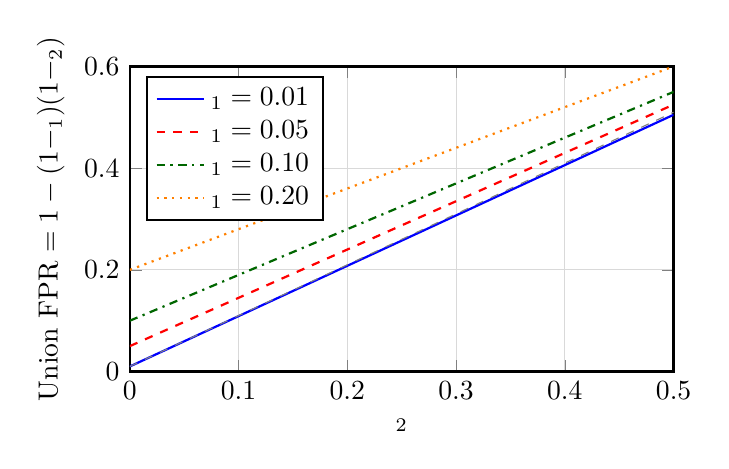
\begin{tikzpicture}
\begin{axis}[
	width=0.7\textwidth,
	height=0.45\textwidth,
	xlabel={$\fprate_2$},
	ylabel={Union FPR $= 1 - (1-\fprate_1)(1-\fprate_2)$},
	xmin=0, xmax=0.5,
	ymin=0, ymax=0.6,
	legend pos=north west,
	ymajorgrids, xmajorgrids,
	major grid style={gray!30},
	thick,
	samples=100,
	domain=0:0.5,
]
\addplot[blue, solid] {1-(1-0.01)*(1-x)};
\addlegendentry{$\fprate_1 = 0.01$}
\addplot[red, dashed] {1-(1-0.05)*(1-x)};
\addlegendentry{$\fprate_1 = 0.05$}
\addplot[black!60!green, dashdotted] {1-(1-0.10)*(1-x)};
\addlegendentry{$\fprate_1 = 0.10$}
\addplot[orange, dotted, thick] {1-(1-0.20)*(1-x)};
\addlegendentry{$\fprate_1 = 0.20$}
\addplot[gray, thin, dashed, forget plot] {x + 0.01};
\end{axis}
\end{tikzpicture}
\caption{Union false positive rate
$\fprate = 1 - (1-\fprate_1)(1-\fprate_2)$ as a function of $\fprate_2$
for several fixed values of $\fprate_1$.
The thin dashed gray line shows the additive approximation
$\fprate_1 + \fprate_2$ for $\fprate_1 = 0.01$;
for small rates, the union FPR is nearly additive, but the
product term $\fprate_1 \fprate_2$ becomes significant as rates grow.
By De Morgan duality, the intersection FNR has the same functional form
with $\fnrate_i$ replacing $\fprate_i$.}
\label{fig:union_fpr}
\end{figure}

\begin{example}[Numerical illustration of union error rates]
\label{ex:numerical_union}
Let $|U| = 1000$, $|A_1| = 100$, $|A_2| = 80$, and $|A_1 \cap A_2| = 30$.
Then $|A_1 \cup A_2| = 100 + 80 - 30 = 150$ and the partition weights for the union (\cref{eq:union_weights}) are
\begin{equation}
w_1 = \frac{70}{150} \approx 0.467, \quad
w_2 = \frac{50}{150} \approx 0.333, \quad
w_3 = \frac{30}{150} = 0.200.
\end{equation}
Suppose $\fprate_1 = 0.01$, $\fprate_2 = 0.02$, $\fnrate_1 = 0.05$, and $\fnrate_2 = 0.03$.
By \cref{thm:union_fprate}, the union FPR is
\begin{equation}
\fprate = 1 - (1 - 0.01)(1 - 0.02) = 1 - 0.99 \times 0.98 = 0.0298.
\end{equation}
By \cref{thm:union_fnrate}, the union FNR is
\begin{align}
\fnrate &= 0.467 \times 0.05 \times (1 - 0.02)
         + 0.333 \times 0.03 \times (1 - 0.01)
         + 0.200 \times 0.05 \times 0.03 \notag \\
       &= 0.02288 + 0.00990 + 0.00030 = 0.03308.
\end{align}
Thus $\tilde{A}_1 \cup \tilde{A}_2$ is a Bernoulli set approximating $A_1 \cup A_2$ with FPR $\approx 0.030$ and FNR $\approx 0.033$.
\end{example}

Several structural observations follow from the table.

The union and intersection formulas exhibit a duality:
the false positive rate of the union has the same functional form as the
false negative rate of the intersection, and vice versa.
This duality reflects De Morgan's laws: $A_1 \cup A_2 =
\SetComplement[\SetComplement[A_1] \cap \SetComplement[A_2]]$, so that
the union may be realized by complementing both operands, intersecting,
and complementing the result.
By \cref{thm:complement_rates}, each complementation exchanges the roles
of $\fprate$ and $\fnrate$, producing the observed symmetry.

\subsection{Closure properties}
\label{sec:closure}
The error rates in \cref{tab:set_ops} reveal that certain classes of
Bernoulli sets are closed under specific operations.

\begin{theorem}[Closure of positive Bernoulli sets under intersection]
\label{thm:closure_positive_intersect}
If $\tilde{A}_1$ and $\tilde{A}_2$ are positive Bernoulli sets, then
$\tilde{A}_1 \cap \tilde{A}_2$ is a positive Bernoulli set.
\end{theorem}
\begin{proof}
By \cref{cor:intersect_positive}, when $\fnrate_1 = \fnrate_2 = 0$,
the intersection has $\fnrate = 0$ and
$\fprate = w_1 \fprate_2 + w_2 \fprate_1
+ w_3 \fprate_1 \fprate_2 \geq 0$.
Since $\fnrate = 0$, the result is a positive Bernoulli set.
\end{proof}

\begin{theorem}[Closure of negative Bernoulli sets under union]
\label{thm:closure_negative_union}
If $\tilde{A}_1$ and $\tilde{A}_2$ are negative Bernoulli sets, then
$\tilde{A}_1 \cup \tilde{A}_2$ is a negative Bernoulli set.
\end{theorem}
\begin{proof}
By \cref{cor:union_negative}, when $\fprate_1 = \fprate_2 = 0$,
the union has $\fprate = 0$ and
$\fnrate = w_1 \fnrate_1 + w_2 \fnrate_2
+ w_3 \fnrate_1 \fnrate_2 \geq 0$.
Since $\fprate = 0$, the result is a negative Bernoulli set.
\end{proof}

\begin{remark}
Complement maps positive Bernoulli sets to negative Bernoulli sets and vice
versa by \cref{thm:complement_rates}.
In particular, the closure of positive sets under intersection and the
closure of negative sets under union are dual statements: applying
De Morgan's law and complementation converts one into the other.
\end{remark}

These closure properties constrain which expressions over Bernoulli sets
produce outputs that remain within the positive or negative class.
The following grammar characterizes the set-theoretic expressions that are
guaranteed to produce a positive Bernoulli set (production $\langle
\mathrm{exp} \rangle$) or a negative Bernoulli set (production $\langle
\mathrm{nexp} \rangle$):
\begin{align}
\label{eq:grammar_exp}
\langle \mathrm{exp} \rangle \; ::= \; &
    \langle \mathrm{aset} \rangle
    \;\mid\; \langle \mathrm{exp} \rangle \cup \langle \mathrm{exp} \rangle
    \;\mid\; \langle \mathrm{exp} \rangle \cap \langle \mathrm{exp} \rangle
    \;\mid\; \SetComplement[\langle \mathrm{nexp} \rangle] \\
\label{eq:grammar_nexp}
\langle \mathrm{nexp} \rangle \; ::= \; &
    \langle \mathrm{naset} \rangle
    \;\mid\; \langle \mathrm{nexp} \rangle \cup \langle \mathrm{nexp}
        \rangle
    \;\mid\; \langle \mathrm{nexp} \rangle \cap \langle \mathrm{nexp}
        \rangle
    \;\mid\; \SetComplement[\langle \mathrm{exp} \rangle]
\end{align}
where $\langle \mathrm{aset} \rangle$ denotes a positive Bernoulli set and
$\langle \mathrm{naset} \rangle$ denotes a negative Bernoulli set.

The grammar is justified as follows.
A union of positive Bernoulli sets is positive by
\cref{cor:union_positive}, and an intersection of positive sets is positive
by \cref{thm:closure_positive_intersect}; both productions are therefore included.
Since $A_1 \cap A_2 = \SetComplement[\SetComplement[A_1] \cup
\SetComplement[A_2]]$, the intersection of two positive sets may be
expressed as the complement of a union of two negative sets (via
\cref{thm:complement_rates}), which by
\cref{thm:closure_negative_union} is negative, and whose complement is
therefore positive.
The dual argument applies for the $\langle \mathrm{nexp} \rangle$
production.

\subsection{Asymptotic behavior of composed error rates}

The error-rate formulas above determine the \emph{expected} rates for composed approximate sets.
Since these composed rates inherit the Bernoulli structure from their operands, the asymptotic normal approximation of \cref{sec:asymtotic} applies.

For example, the true negative rate of the union $\tilde{A}_1 \cup \tilde{A}_2$ has the asymptotic distribution
\begin{equation}
\TNR_\n \sim \normdist\!\left(\tnrate_1 \tnrate_2, \frac{\tnrate_1 \tnrate_2 (1-\tnrate_1 \tnrate_2)}{\n}\right),
\end{equation}
where $\n = u - |A_1 \cup A_2|$ is the number of negatives.
As $\n \to \infty$, the distribution converges in probability to $\tnrate_1 \tnrate_2$.

\begin{remark}[Convergence of intersections of positive approximate sets]
	Consider a sequence $\PASet{A}[\fprate_1],\ldots,\PASet{A}[\fprate_n]$ of independent positive approximate sets of the same objective set.
	As $n \to \infty$, $\bigcap_{i=1}^{n} \PASet{A}[\fprate_i]$ converges almost surely to $\Set{A}$, since each negative element survives with probability $\prod_{i=1}^{n} \fprate_i \to 0$.
	Dually, for negative approximate sets, $\bigcup_{i=1}^{n} \NASet{A}[\fnrate_i]$ converges almost surely to $\Set{A}$.
\end{remark}

\begin{remark}[Monoidal structure]
\label{rem:monoid}
The results above show that the collection of Bernoulli sets over $U$ is
closed under union and intersection (with computable output rates).
Since these operations inherit associativity and commutativity from the
powerset $2^U$, Bernoulli sets form a commutative semigroup under each.
If the degenerate-case axiom is adopted---$\Prob{\ASet{\EmptySet} =
\EmptySet} = 1$ and, dually, $\Prob{\ASet{U} = \Set{U}} = 1$ (see
\cref{sec:higher_order_model})---then $\EmptySet$ and $\Set{U}$ serve as
identity elements, yielding commutative monoids under union and
intersection respectively.
This is useful in practice: the $n$-ary union
$\bigcup_{i=1}^{n} \ASet{A}_i$ (as arises in approximate Boolean search,
\cref{sec:bool_search}) is precisely the monoidal fold, requiring only an
associative operation and an identity element.
\end{remark}
